\documentclass[../manifest.tex]{subfiles}

% - should include scenarios of use and multiple screenshots of your software in action. walk the reader through how your interface succeeds (or acknowledge how it falls short) in solving the intended problem.
% - if you did any evaluation (deployment to target users, computational benchmarks), do report on that here.

\begin{document}

Teamline was designed specifically for the use-case of supporting teaching assistants ('TAs') in grading students for the course 'CPSC 310 Introduction to Software Engineering' at the University of British Columbia\footnote{See section TODO for elaboration on how the domain can be extended.}. The course is characterized by multiple deliverables and a retrospective session after each deliverable with the TA and each team member individually. Students are required to hand in an individual contribution file for each deliverable that points out how they contributed to their implementation, outlining their major commits and evaluating what went well or bad during the 'sprint'. Figure~\ref{fig:sample-contribution-file} shows an example contribution file.

\begin{figure}[h]
  \centering
  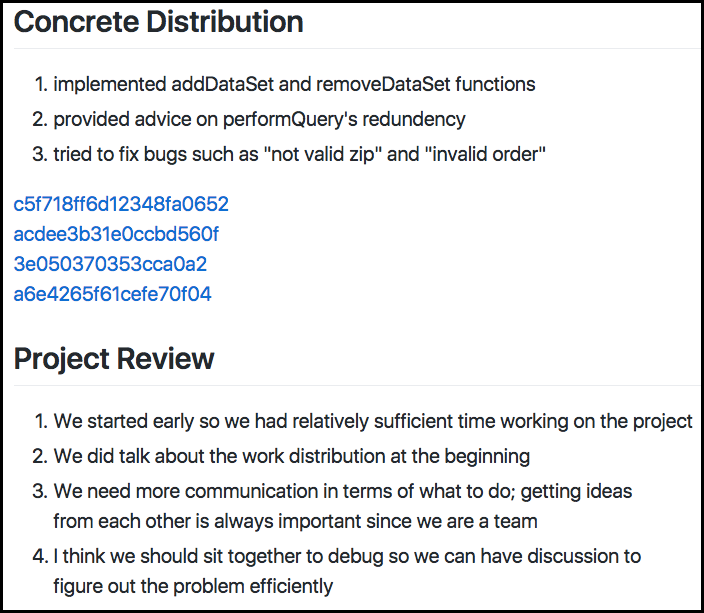
\includegraphics[width=\linewidth]{sample-contribution-file}
  \caption{Sample contribution file}
  \label{fig:sample-contribution-file}
\end{figure}

Using this contribution file as a basis, the TA will then talk to the team members and try to assess if they contributed evenly to the deliverable. The TA may use information provided by Github, like the deliverable's commit history and contribution graphs (see Figure~\ref{fig:sample-contribution-graph}) to obtain a better picture for the assessment. If an uneven contribution is visible, the TA is then to downscale the team member who contributed less gradually. As described earlier, this assessment can be a very challenging task with only the information provided.

\begin{figure}[h]
  \centering
  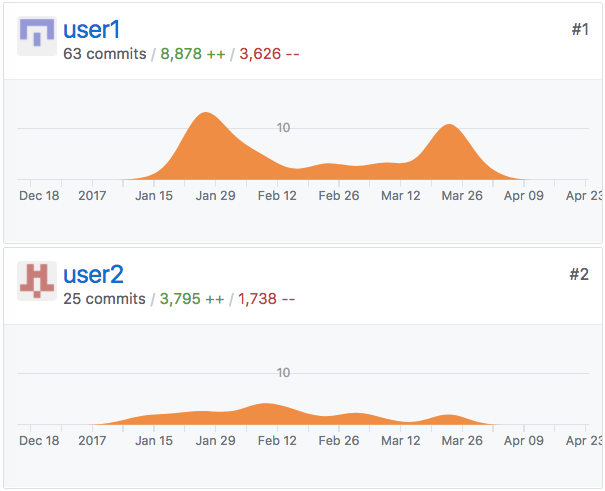
\includegraphics[width=\linewidth]{sample-contribution-graph}
  \caption{Sample contribution graph}
  \label{fig:sample-contribution-graph}
\end{figure}



\end{document}
